\subsection{Initial boundary problem}

\begin{frame}{Initial boundary problem}
  \begin{description}
    \item[Dane:]
      \begin{itemize}
        \item stała $a>0$
        \item trzy ciągłe funkcje: $g_1(t)$, $g_2(t)$, $f(x)$ dla $ \left\{ \begin{array}{l} t \ge 0 \\ 0 \le x \le a \end{array} \right. $
      \end{itemize}
    \item[Szukana:]
      $u(x,t)$:
      \begin{itemize}
        \item określona i ciągła \\ dla $0 \le x \le a, t \ge 0$,
        \item spełniająca $(\ref{7})$ \\ dla $0 < x < a, t > 0$,
        \item spełniająca:
        $$ \left\{ \begin{array}{lrl}
        u(x,0) = f(x), & 0 \le x \le a & \text{initial condition} \\
        u(0,t) = g_1(t), & t \ge 0 & \text{boundary condition} \\
        u(a,t) = g_2(t), & t \ge 0 & \text{boundary condition}
        \end{array} \right. $$
      \end{itemize}
  \end{description}
\end{frame}

\begin{frame}
  \centerline{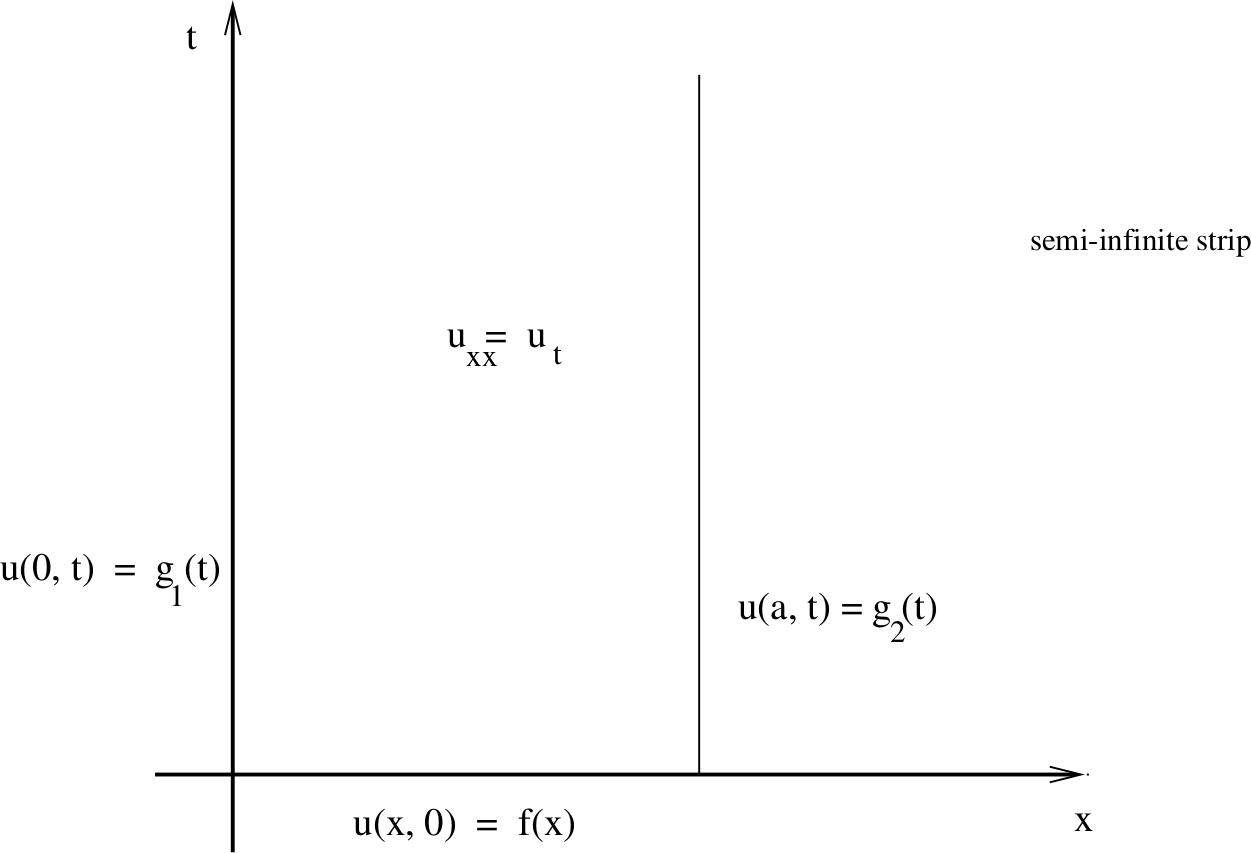
\includegraphics[height = 0.85 \textheight]{img/23/ibp}}
\end{frame}

\begin{frame}
  Rozwiązanie $\rightarrow$ szeregi Fouriera

  \begin{alertblock}{Problem}
    Ten sam problem jak poprzednio...
  \end{alertblock}
\end{frame}
